\documentclass[a4paper, 11pt]{book}

\usepackage[main=spanish,japanese]{babel}
\usepackage[utf8]{inputenc}
\usepackage{CJKutf8} % Para poder escribir caracteres CJK
\usepackage{tcolorbox} % Para la caja de explicacion rapida
\usepackage{graphicx} % Para imagenes
\usepackage{hyperref} % Para permitir que el indice sea clicable.
\usepackage{tabularx} % Para poder tener saltos de lineas automaticos en las tablar
                                          % En caso de desearlo dar medidas especificas a cada tabla.

\usepackage[overlap, CJK]{ruby} % Paquete necesario para poder añadir furigana

% Si se desea cambiar la distancia entre el furigana y la palabra ajustar aqui.
\renewcommand{\rubysep}{0ex}

% Ajustar el tamaño del texto en furigana. La dimension basicamente es el tamaño base
% por el escalado a aplicar. Si se pone a 1 el tamaño del furigana sera el mismo que el del
% texto del cuerpo.
\renewcommand{\rubysize}{0.6}
\setcounter{tocdepth}{4}

\definecolor{celeste}{HTML}{E0F7FA}

\title {
	Apuntes de gramática \\ 
	\large \emph {Mi subtitulo} % Si se desea se puede usar el paquete titling en vez de esto.
}
\author{Nombre}

%% ----------------------------------------------
% Comando para insertar texto en japones en cualquier
% momento que desee el escritor.
%
% Parametros:
% 	* El unico argumento es el texto en japones a mostrar.
%% ----------------------------------------------
\newcommand{\tjp}[1]{
	\begin{CJK}{UTF8}{min}
		#1
	\end{CJK}
}

%% ----------------------------------------------
% Comando para insertar texto en japones con furigana
% cuando lo asi lo desee el autor.
%
% Parametros:
% 	* El texto base a escribir sobre el cual se pondrá furigana.
%   * El furigana a escribir sobre la palabra base.
%% ----------------------------------------------
\newcommand{\tjpf}[2]{
	\begin{CJK}{UTF8}{min}
		\ruby{#1}{#2}
	\end{CJK}
}

%% ----------------------------------------------
% Igual que el comando anterior sin establecer el CJK
% esto hace que en entornos donde ya se tiene CJK
% no se vuelva a definir. Como ejemplos, precedencia,
% o definiciones rapidas
%
% Parametros:
% 	* El texto base a escribir sobre el cual se pondrá furigana.
%   * El furigana a escribir sobre la palabra base.
%% ----------------------------------------------
\newcommand{\tjpfn}[2]{
	\ruby{#1}{#2}
}

%% ----------------------------------------------
% Comando para insertar un ejemplo en japones.
% Se constituye de dos argumentos, la parte en japones
% y su traducción al español.
%
% Parametros:
% 	* El primero argumento es el texto japones del ejemplo.
% 	* El segundo argumento es su tradución al español.
%% ----------------------------------------------
\newcommand{\jpex}[2] {
	\vspace{1.0\baselineskip}
	\begin{CJK}{UTF8}{min}
		\noindent\textbf{\large{#1}}
		$\rightarrow$ \emph{#2}
	\end{CJK}
}

\newcommand{\jpexn}[2] {
	\vspace{1.0\baselineskip}
	\noindent\textbf{\large{#1}}
	$\rightarrow$ \emph{#2}
}

%% ----------------------------------------------
% Comando para indicar las formas gramaticales
% que preceden a cierta forma gramatical
%
% Parametros:
% 	* El primero argumento es las formas gramaticales que preceden
%		a la forma gramatical tratada.
% 	* El segundo argumento es la forma gramatical en cuestion.
%% ----------------------------------------------
\newcommand{\grpre}[2]{
	\begin{center}
		\begin{CJK}{UTF8}{min}
			\begin{tabular}{l}
				#1
			\end{tabular}
			$+$
			\begin{tabular}{l}
				#2
			\end{tabular}
		\end{CJK}
	\end{center}
}

\newcommand{\grpren}[2]{
	\begin{center}
		\begin{tabular}{l}
			#1
		\end{tabular}
		$+$
		\begin{tabular}{l}
			#2
		\end{tabular}
	\end{center}
}

%% ----------------------------------------------
% Seccion donde aparece la deficion rapida de una expresion
% gramatical. 
%
% Parametros:
% 	* Argumento opcional entre [] que servira de titulo de la caja.
%% ----------------------------------------------
\newenvironment{defrapida}[1][\unskip]{
	\noindent
	\begin{CJK}{UTF8}{min}
		\begin{tcolorbox}[colback=celeste, title=#1]
} {
		\end{tcolorbox}
	\end{CJK}
}

\newenvironment{defrapidan}[1][\unskip]{
	\noindent
	\begin{tcolorbox}[colback=celeste, title=#1]
	} {
	\end{tcolorbox}
}

\begin{document}
	\maketitle
	\tableofcontents
	\listoftables
	\listoffigures
	
	% Para mas comodidad se puede declarar todo el documento como \begin{CJK}{UTF8}{min} \ end{CJK}
	% En caso de hacer esto usar los entornos y comandos que se llaman igual a los anteriores
	% pero finalizados en la letra n. Esto indica que nmo se vuelve a declarar el entorno CJK en su interior.

	%%%%%%%%%%%%%%%%%%%%%%%%%%%%
	%% Contenido de ejemplo eliminar para el uso.	%
	%%%%%%%%%%%%%%%%%%%%%%%%%%%%

	% Importante usar protect para que se definan correctamente en el .toc
	% los titulos usando caracteres CJK. Si no se usa protect cuando se usa tjp
	% en un titulo que aparece en el indice los que vengan a continuacion no
	% funcionaran.
	\chapter{\protect\tjp{始めましょう!}}
	\section{Ejemplo sección}
	\subsection{Ejemplo subsección}
	
	Hola buenos dias!!! \tjp{こんにちは!} Este texto es de prueba para ver como se ve con salto de linea \tjpf{助詞}{じょし} incluso con furigana. \tjpf{自動販売機}{じどうはんばいき}
	
	% hbt! por si se quiere que aparezca en linea con el texto
	\begin{figure}[hbt!]
		\centering
		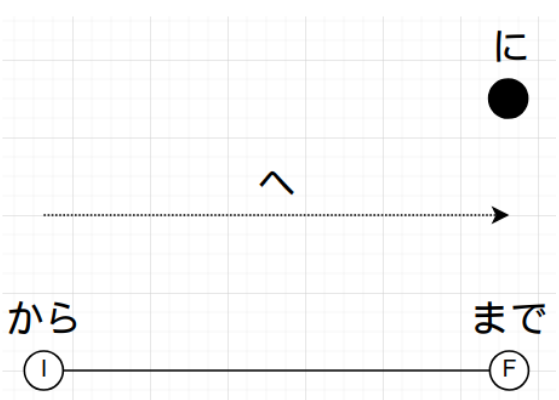
\includegraphics[width=0.5\textwidth]{ExampleFigures/ejemplo-diferencia-grafica-ni-kara-made-he.png}
		\caption{Diferencias entre \tjp{から・まで、に y へ}}
	\end{figure}
	
	\begin{table}[hbt!]
		\centering
		\begin{tabularx}{\textwidth}{| l | c | X |}
			\hline
			\textbf{\tjp{助詞}} & \textbf{Lectura} & \textbf{Uso principal} \\
			\hline
			\tjp{は} & Wa & Indica el tema principal de la frase \\
			\tjp{が} & Wa & Indica el sujeto de la frase \\
			\tjp{を} & O & Indica el objeto directo de la acción (quien la recibe) \\
			\tjp{に} & Wa & Indica direccion, tiempo, lugar. (muchas veces le sujeto indirecto) \\
			\hline
		\end{tabularx}
		\caption{Varias particulas (\tjp{助詞})}
	\end{table}
	
	\grpre{
		Sustantivo+だ \\ Verbo informal \\ Adjetivo-な
	} {
		例えば
	}

	\chapter{Ejemplo titulo}

	Esta es una explicacion de ejemplo de algun concepto gramatical del \tjp{日本語}.

	\begin{defrapida}[Prueba de definicion 例えば]
		Esto es una prueba 例えば
	\end{defrapida}
	
	\begin{defrapida}
		Esto es una prueba 例えば
	\end{defrapida}

	\textbf{EJEMPLOS: }

	\jpex{
		私は\tjpfn{吉良吉影}{きらよしかげ}です。
	}{
		Soy Kira yoshikage.
	}
	
	\jpex{
		私は吉良吉影です。
	}{
		Soy Kira yoshikage.
	}
	
	\begin{table}
		\centering
		\begin{tabularx}{\textwidth}{| l | c | X |}
			\hline
			\textbf{\tjp{助詞}} & \textbf{Lectura} & \textbf{Uso principal} \\
			\hline
			\tjp{は} & Wa & Indica el tema principal de la frase \\
			\tjp{が} & Wa & Indica el sujeto de la frase \\
			\tjp{を} & O & Indica el objeto directo de la acción (quien la recibe) \\
			\tjp{に} & Wa & Indica direccion, tiempo, lugar. (muchas veces le sujeto indirecto) \\
			\hline
		\end{tabularx}
		\caption{Varias particulas segundo ejemplo (\tjp{助詞})}
	\end{table}
	
	\begin{figure}
		\centering
		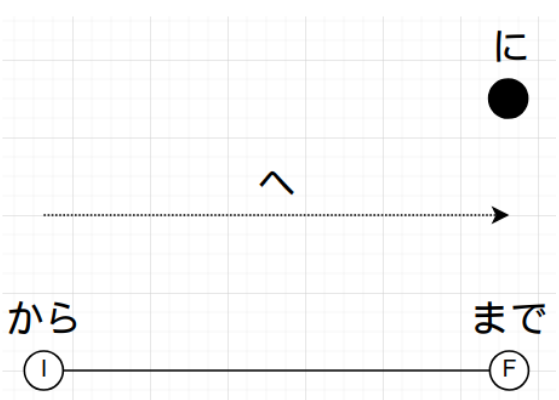
\includegraphics[width=0.5\textwidth]{ExampleFigures/ejemplo-diferencia-grafica-ni-kara-made-he.png}
		\caption{Diferencias entre \tjp{から・まで、に y へ} segunda imagen.}
	\end{figure}

	% Actualizar el numero de bibliografias a las deseadas
	\begin{thebibliography}{7}
		\bibitem{lamport94}
		Leslie Lamport,
		\textit{\LaTeX: a document preparation system},
		Addison Wesley, Massachusetts,
		2nd edition,
		1994.
		
		\bibitem{taekim14}
		Tae Kim,
		\textit{A Guide to Japanese Grammar. A Japanese approach to learning Japanese grammar},
		CreateSpace Independent Publishing Platform,
		2014.
	\end{thebibliography}

\end{document}

